\subsection{RNA Synthesis}\label{sec:RNA_synthesis}
With the machinery governing the replication of the genome accounted for, we
now turn our attention to the next stage of the central dogma -- the
transcription of DNA to form RNA. We primarily consider three major groupings
of RNA, namely the RNA associated with ribosomes (rRNA), the RNA encoding the
amino-acid sequence of proteins (mRNA), and the RNA which links codon
sequence to amino-acid identity during translation (tRNA). Despite the varied
function of these RNA species, they share a commonality in that they are
transcribed from DNA via the action of RNA polymerase. In the coming
paragraphs, we will consider the synthesis of RNA as a rate limiting step in
bacterial division by estimating how many RNA polymerases must be present to
synthesize all necessary rRNA, mRNA, and tRNA.

\subsubsection{rRNA}
We begin with an estimation of the number of RNA polymerases needed to
synthesize the rRNA that serve as catalytic and structural elements of the
ribosome. Each ribosome contains three rRNA molecules of lengths 120, 1542,
and 2904 nucleotides (BNID: 108093), meaning each ribosome
contains $\approx$ 4500 nucleotides. As the \textit{E. coli} RNA polymerase
transcribes DNA to RNA at a rate of $\approx$ 40 nucleotides per second
(BNID: 101904), it takes a single RNA polymerase
$\approx$ 100 s to synthesize the RNA needed to form a single functional ribosome.
Therefore, in a 5000 s division time, a single RNA polymerase transcribing
rRNA at a time would result in only $\approx$ 50 functional ribosomal rRNA
units -- far below the observed number of $\approx 10^4$ ribosomes per cell.

Of course, there can be more than one RNA polymerase transcribing the rRNA genes
at any given time. To elucidate the \textit{maximum} number of rRNA units that can
be synthesized given a single copy of each rRNA gene, we will consider a
hypothesis in which the rRNA operon is completely tiled with RNA polymerase.
\textit{In vivo} measurements of the kinetics of rRNA transcription have revealed that
RNA polymerases are loaded onto the promoter of an rRNA gene at a rate of
$\approx$ 1 per second (BNID: 111997, 102362). If RNA
polymerases are being constantly loaded on to the rRNA genes at this rate,
then we can assume that $\approx$ 1 functional rRNA unit is
synthesized per second. With a 5000 second division time, this hypothesis
leads to a maximal value of 5000 functional rRNA units, still undershooting
the observed number of $10^4$ ribosomes per cell.

\textit{E. coli}, like many other bacterium, have evolved a clever mechanism to surpass this kinetic limit
for the rate of rRNA production. Rather than having only one copy of each rRNA
gene, \textit{E. coli} has seven copies of the operon (BIND: 100352) four of which are localized directly adjacent to the origin of
replication \citep{birnbaum1971}. As fast growth also implies an increased gene
dosage due to parallellzed chromosomal replication, the total number of rRNA
genes can be on the order of $\approx$ 10 -- 70 copies at moderate to fast
growth rates \citep{stevenson2004}. Given a 5000
second division time, we can make the lower-bound estimate that the typical cell
will have $\approx$ 7 copies of the rRNA operon. Synthesizing one functional rRNA unit per
second per rRNA operon, a total of $5 \times 10^4$ rRNA units can be
synthesized, comfortably above the observed number of ribosomes per cell.

How many RNA polymerases are then needed to constantly transcribe 7 copies of
the rRNA genes? We approach this estimate by considering the maximum number
of RNA polymerases tiled along the rRNA genes with a loading rate of 1 per
second and a transcription rate of 40 nucleotides per second. Considering
that a RNA polymerase has a physical footprint of approximately 40
nucleotides (BNID: 107873), we can expect
$\approx$ 1 RNA polymerase per 80 nucleotides. With a total length of
$\approx$ 4500 nucleotides per operon and 7 operons per cell, the maximum
number of RNA polymerases that can be transcribing rRNA at any given time is
$\approx$ 500. As we will see in the coming sections, the
synthesis of rRNA is the dominant requirement of the RNA polymerase pool.

\subsubsection{mRNA}
To form a functional protein, all protein coding genes must first be
transcribed from DNA to form an mRNA molecule. While each protein requires an
mRNA blueprint, many copies of the protein can be synthesized from a single
mRNA. Factors such as strength of the ribosomal binding site, mRNA stability,
and rare codon usage frequency dictate the number of proteins that can be
made from a single mRNA, with yields ranging from 10$^1$ to 10$^4$ (BNID: 104186; 100196;
106254). Computing the geometric mean of this range yields
$\approx$ 1000 proteins synthesized per mRNA, a value that agrees with
experimental measurements of the number of proteins per cell ($\approx 3
\times 10^6$, BNID: 100088) and total number of mRNA per
cell ($\approx 3 \times 10^3$, BNID:100064).

This estimation captures the \textit{steady-state} mRNA copy number, meaning
that at any given time, there will exist approximately 3000 unique mRNA
molecules. To determine the \textit{total} number of mRNA that need to be
synthesized over the cell's lifetime, we must consider degradation of the mRNA.
In most bacteria, mRNAs are rather unstable with life times on the order of
several minutes (BNID: 104324; 106253; 111927; 111998). For
convenience, we assume that the typical mRNA in our cell of interest has a
typical lifetime of $\approx$ 300 seconds. Using this value, we can determine
the total mRNA production rate to maintain a steady-state copy number of 3000
mRNA per cell. While we direct the reader to the appendix for a more detailed
discussion of mRNA transcriptional dynamics, we state here that the total mRNA
production rate must be on the order of $\approx$ 15 mRNA per second. In
\textit{E. coli}, the average protein is $\approx$ 300 amino acids in length
(BNID: 108986), meaning that the corresponding mRNA is
$\approx$ 900 nucleotides which we will further approximate as $\approx$ 1000
nucleotides to account for the non-protein coding regions on the 5' and
3' ends. This means that the cell must have enough RNA polymerase molecules
about to sustain a transcription rate of $\approx 1.5 \times 10^4$ nucleotides
per second. Knowing that a single RNA polymerase polymerizes RNA at a clip of 40
nucleotides per second, we arrive at a comfortable estimate of $\approx$ 250 RNA
polymerase complexes needed to satisfy the mRNA demands of the cell. It is worth
noting that this number is approximately half of that required to synthesize
enough rRNA, as we saw in the previous section. We find this to be a striking
result as these 250 RNA polymerase molecules are responsible for the
transcription of the $\approx$ 4000 protein coding genes that are not ribosome
associated.

\subsubsection{tRNA}
The final class of RNA molecules worthy of quantitative consideration are the
tRNAs that are used during translation to map codon sequence on mRNA to specific amino acids.
Unlike mRNA or rRNA, each individual tRNA is remarkably short, ranging
from 70 to 95 nucleotides each (BNID: 109645; 102340). What
they lack in length, they make up for in abundance, with reported values ranging from
$\approx$5$\times$10$^4$ (BNID: 105280) to
$\approx$5$\times$10$^5$ (BNID: 108611). To test tRNA synthesis as a possible
growth-rate limiting stage, we will err towards a higher abundance of $\approx$
5$\times$10$^5$ per cell. Combining the abundance and tRNA length measurements,
we make the estimate that $\approx 5 \times 10^7$ nucleotides are sequestered in tRNA per cell.
Unlike mRNA, tRNA is remarkably stable with typical lifetimes \textit{in vivo}
on the order of $\approx$ 48 hours \citep{abelson1974,svenningsen2017} -- well
beyond the timescale of division. Once again using our rule-of-thumb for the
rate of transcription to be 40 nucleotides per second and assuming a division
time of $\approx$ 5000 seconds, we arrive at an estimate of $\approx$ 200 RNA
polymerases to synthesize enough tRNA. This requirement pales in comparison to
the number of polymerases needed to generate the rRNA and mRNA pools and can be
neglected as a significant transcriptional burden.

\begin{figure}
    \begin{fullwidth}
    \centering{
        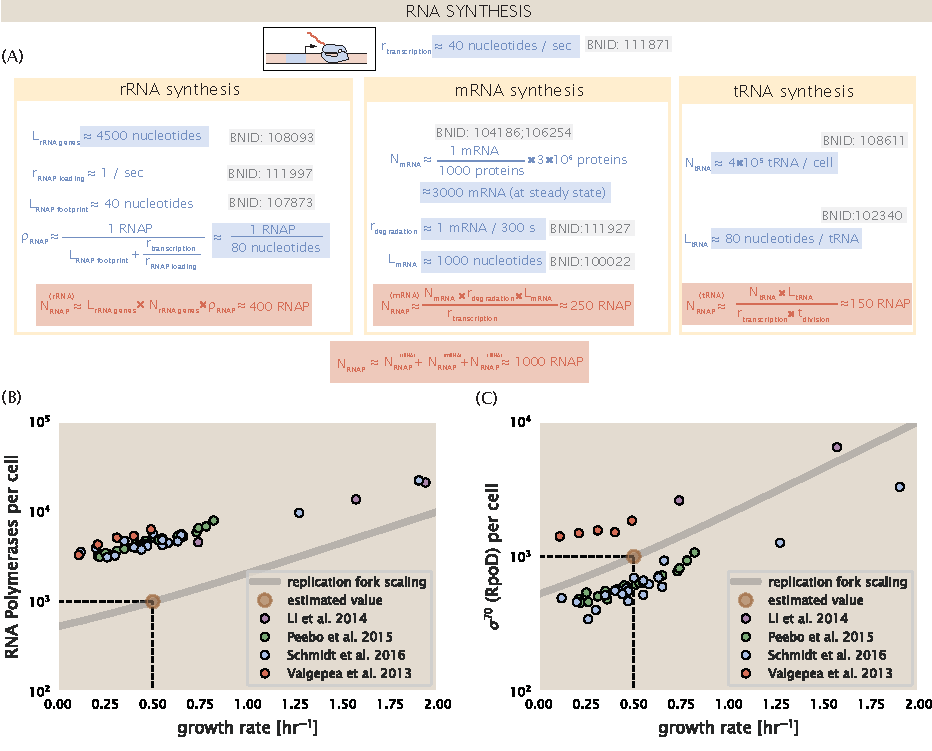
\includegraphics{main_figs/fig7_RNA_synthesis.pdf}
        \caption{\textbf{Estimation of the RNA polymerase demand and
        comparison with experimental data.} (A) Estimations for the number of
        RNA polymerase needed to synthesize sufficient quantities of rRNA, mRNA,
        and tRNA from left to right, respectively.(B) The RNA
        polymerase core enzyme copy number as a function of growth rate. Colored
        points correspond to the average number RNA polymerase core enzymes that
        could be formed given a subunit stoichiometry of [RpoA]$_2$[RpoC][RpoB].
        (C) The abundance of $\sigma^{70}$ as a function of growth rate.
        Estimated value for the number of RNAP is shown in (B) and (C) as a
        translucent brown point at a growth rate of 0.5 hr$^{-1}$.}
    \label{fig:RNA_synthesis}
    }
    \end{fullwidth}
\end{figure}


\subsubsection{RNA Polymerase and $\sigma$-factor Abundance}
These estimates, summarized in \FIG{RNA_synthesis} (A), reveal that synthesis of
rRNA  and mRNA are the dominant RNA species synthesized by RNA polymerase,
suggesting the need for $\approx$ 1000 RNA polymerases per cell. As is revealed
in \FIG{RNA_synthesis} (B), this estimate is about an order of magnitude below
the observed number of RNA polymerase complexes per cell ($\approx$ 5000 -
7000). The difference between the estimated number of RNA polymerase needed for
transcription and and
these observations are consistent with recent literature revealing that
$\approx$ 80 \% of RNA polymerases in \textit{E. coli} are not transcriptionally
active \citep{patrick2015}. Our estimate ignores the possibility that some
fraction is only nonspecifically bound to DNA, as well as the obstacles that RNA
polymerase and DNA polymerase present for each other at they move along the DNA
\citep{finkelstein2013}.

In addition, it is also vital to consider the role of $\sigma$-factors which
help RNA polymerase identify and bind to transcriptional start sites
\citep{browning2016}. Here we consider $\sigma^{70}$ (RpoD) which is the
dominant "general-purpose" $\sigma$-factor in \textit{E. coli}. While initially
thought of as being solely involved in transcriptional initiation, the past two
decades of single-molecule work has revealed a more multipurpose role for
$\sigma^{70}$ including facilitating transcriptional elongation
\citep{kapanidis2005, goldman2015, perdue2011,mooney2003,mooney2005}.
\FIG{RNA_synthesis} (B) is suggestive of such a role as the number of
$\sigma^{70}$ proteins per cell is in close agreement with our estimate of the
number of transcriptional complexes needed.

These estimates provide insight as to the observed magnitude of both RNA
polymerase and the $\sigma$-70 factor. As we have done in the previous sections,
and described in Appendix \nameref{sec:SI_continuum_est}, we can generalize these estimates
across a wide range of growth rates (grey line in \FIG{RNA_synthesis}(B). While
there remains some disagreement in the magnitude of the copy number, this
estimate appears to very adequately describe the growth rate dependence of these
complexes. Furthermore, these findings illustrate that transcription
cannot be the rate limiting step in bacterial division. \FIG{RNA_synthesis} (A)
reveals that the availability of RNA polymerase is not a limiting factor for
cell division as the cell always has an apparent $\sim$ 10-fold excess than needed.
Furthermore, if more transcriptional activity was needed to satisfy the cellular
requirements, more $\sigma^{70}$-factors could be expressed to utilize a larger
fraction of the RNA polymerase pool.
